\documentclass[12pt,answers,addpoints]{exam}
\usepackage{float} %  figure inside minipage 
\usepackage{ifthen,empheq}
\usepackage[]{graphicx}
\usepackage[]{minted}
\usepackage{amssymb}
\usepackage[multidot]{grffile}
\usepackage{pgfplots}
\setlength{\headheight}{20pt}

\usepackage{tikz}
\usepgfplotslibrary{external}
\tikzexternalize[prefix=_tikz/,shell escape=-shell-escape]
\tikzset{external/system call={pdflatex \tikzexternalcheckshellescape -halt-on-error -interaction=batchmode -jobname "\image" "\texsource"}}
\immediate\write18{mkdir -p _tikz}

\title{Solution to HW1}
\usepackage{hyperref}
\printanswers

\begin{document}
\maketitle

\begin{questions}

\question{}

\begin{parts}

\part If $0<a<b$, and c is any real number, rewrite the sets $\{x: a<|x-c|<b\}$ in
terms of intervals.   Do the same for $a=0$, and also give a clear description
in words.  In this case, it will be something like "all the numbers between
[something] and [something else] except for [these one(s)]

\begin{solution}

Its usually a good idea to play with concrete numbers before manipulating the
symbols. For example, which one is correct  $a < b < c$ then $-a > -b > -c$, or
$a < b < c$ then $-a < -b < -c$  etc. This become easy to answer once we notice
that $1 < 2 < 3$ then $ -1 > -2 > -3$. This is just a quick and dirty reality
check rather than replacement of understanding by doing proof. We are going to
use this simple fact.

We have, $ \{ x : a < | x - c | < b \}$ which means $a < x - c < b,
\text{when}\; x > c$, and $a < c - x < b, \text{when}\; x < c$. The later can
be rewritten as $-a > x -c > -b$. 

For two different cases ($x > c$, and $x < c$), we have the following:
\begin{align}
    a &< x - c < b  &(a + c < x < b + c) \\
    -a &> x -c < -b &(-a +c < x < -b +c)
\end{align}

Now we can use {\bf intervals } to rewrite it i.e. $x = { (a+c, b+c) \cup
(-a+c,-b+c) }$.

See the figure \ref{fig:1a}. Code is available
\href{https://github.com/dilawar/Courses/blob/master/Calculus2016/Homework1/sol1_a.py}{here}.

\begin{figure}[H]
    \includegraphics[width=\columnwidth]{./sol1_a.py.png}
    \caption{Numerical solution to problem 1(a)}
    \label{fig:1a}
\end{figure}

\end{solution}


\part 
Given $a<b$ real numbers, describe the intervals $(a,b)$ using the
absolute value function.  That is, write $(a,b)=\{x:  ... \}$ where "$\ldots$"
is some condition using absolute value.

\begin{solution}

$(a, b) = \{ x : x > a\; \text{and}\; x < b \}$. How about this,
$ (a, b) = \{ x  : \left| x - \frac{a+b}{2} \right| < \frac{b-a}{2} \}$.  See
the simulation result in figure \ref{fig:1b}.

\begin{figure}[H]
    \includegraphics[width=1\columnwidth]{./sol1_b.py.png}
    \caption{Solution to solution 1(b)}
    \label{fig:1b}
\end{figure}

\end{solution}

\part

Similarly, express $\{a,b\}$, i.e. the set containing precisely the two
(different) numbers a and b (e.g. $\{-14.7, e+\pi\}$ or $\{1776,1947\}$ ) using
absolute values. 

\begin{solution}

How about this  $ \{a, b \} = \{ x : [a, a] \cup [b,b] \}$. 
\end{solution}

\end{parts}

\question

\begin{parts}
\part
Show that for any $x, y$, $||x|-|y|| \le |x+y|$.  (This is a useful
counterpart to the triangle inequality and requires a very similar analysis.)

\begin{solution} 

The simulation shown in figure \ref{fig:2a} shows that it is true. The same
picture  picture is plotted in 3d which is more complicated way of saying the
same thing. Showing it is easy using a computational engine but how you gonna
prove it?

\begin{figure}[H]
    \includegraphics[width=1\columnwidth]{./sol2_a.py.png}
    \includegraphics[width=1\columnwidth]{./sol2_a.py_3d.png}
    \caption{ $|x+y|$ is always greater than equal to $||x|-|y||$. A blue dot y-axis
        value represents value of $|x+y|$ while its  x-axis value is value of
        $||x|-|y||$ for a $(x,y)$. Dot falling
        falling over line with slope 1 means that function represented by y-axis is
    larger than the function on x-axis for that particular value of (x, y).}
    \label{fig:2a}
\end{figure}

\end{solution}

\part
Write the set $\{x: |x^2-2x-3|>x\}$ as a union of intervals (i.e. figure out
explicitly for which x this statement is true)

\begin{solution}

First, lets see for what values of $x$, we have $x^2 - 2x - 3$ positive or
negative. We have $(x-3)(x+1)$ as factors. So for $(-\infty, -1] \cup [3,
\infty)$ it is positive and for rest, its negative.

For the positive case $ x^2 - 2x - 3 > x$ and for negative we have $ - x^2 + 2x
+ 3 > x$. Solve for both cases and check if solution lies in the intervals
computed before.

Here is a solution by python script to whet your appetite.

\begin{figure}[H]
\begin{center}
    \includegraphics[width=1\columnwidth]{sol2_b.py.png}
\end{center}
\caption{}
\label{fig:}
\end{figure}

\end{solution}

\end{parts}


% Problem 5.
\question[6] {
    Describe each set as a (union of) interval(s) or as an explicit finite of
    numbers, as appropriate 
}

\begin{parts}

    \part[2] $\{ x \in \mathcal{R}: 3x + 7 = 0 \}$
    \begin{solution}
        $ x = \{ \frac{-7}{3} \} $
    \end{solution}

    \part[2] $\{ x \in \mathcal{R}: \exists a\; \text{such that}\; 3x + 7 = a \}$ 
    \begin{solution}
        $ x = \left\{ x : \frac{a-7}{3},\; \forall a \in \mathcal{R} \right\} =
        \mathcal{R}$.  One to one and onto!
    \end{solution}

    \part[2]  $\{ x \in \mathcal{R}: \exists a\; \text{such that}\; a^2 - 2a = x \}$ 
    \begin{solution}
        $a = 1 \pm \sqrt{ 1 + x}$. For $a$ to be real, $x > -1$. $\{ x : x > -1
        \}$.
    \end{solution}
\end{parts}

%% Problem 6.
\question[10]
\begin{parts}
    \part[2] $|x-1| = |x-2|$ 
    \begin{solution}
        We plot the function $|x-1|-|x-2|$ and find the place where it becomes
        zero. Following is geometrical picture.

        \begin{tikzpicture}[scale=1]
            \begin{axis}[
            xlabel=x,ylabel=$|x-1|-|x-2|$
            , domain=-100:100
            , grid style={draw=gray!20}, grid = both, minor tick num = 4 
            ]
            \addplot [color=blue] { abs(x-1) - abs(x-2) };
            \addplot [color=red] { 0 };
            \end{axis}
        \end{tikzpicture}
        \[   
            |x-1|-|x-2| = 
            \begin{cases}
                x \ge 2 & x-1-x+2 = 1 \\ 
                1 \le x < 2 & x-1-2+x = 2x-3\\
                x < 1 &  1-x-2-x = -1\\
            \end{cases}
        \]
    \end{solution}

    \part[2] $x^2+4|x|+3 = 0$
    \begin{solution}

        \begin{tikzpicture}[scale=1]
            \begin{axis}[
            xlabel=x,ylabel=$x^2+4|x|+3$
            , grid style={draw=gray!20}, grid = both, minor tick num = 1
            ]
            \addplot [color=blue] { x^2+4*abs(x)+3 };
            \addplot [color=red] {  0 };
            \end{axis}
        \end{tikzpicture}
        Answer: $\bf \{\} $
        
    \end{solution}

    \part[2] $x^2-4|x|-3 = 0$
    \begin{solution}

        \begin{tikzpicture}[scale=1]
            \begin{axis}[
            xlabel=x,ylabel=$x^2-4|x|-3$
            , grid style={draw=gray!20}, grid = both, minor tick num = 1
            ]
            \addplot [color=blue] { x^2-4*abs(x)-3 };
            \addplot [color=red] {  0 };
            \end{axis}
        \end{tikzpicture}

        Answer: $\bf \{\} $

    {\bf Note} Previous equation represent a fly butt and this one a human butt.
    A mere change of sign!
    \end{solution}

    \part[2] $|3x-1| < 1$
    \begin{solution}
        \begin{tikzpicture}[scale=1]
            \begin{axis}[
            xlabel=x,ylabel=$|3x-1|$
            , ymax = 2
            , grid style={draw=gray!20}, grid = both, minor tick num = 1
            ]
            \addplot [color=blue] { abs(3*x - 1) };
            \addplot [color=red] { 1 };
            \end{axis}
        \end{tikzpicture}

        Answer: $\bf (0, \frac{2}{3})$. {\bf If you have solved for the case
        $|3x-1| < 0.1$, thats fine too. }
        
    \end{solution}

    \part[2] $3 < \sqrt{2x+1} < 4$
    \begin{solution}
        \begin{tikzpicture}[scale=1]
            \begin{axis}[
                xlabel=x,ylabel=$\sqrt{2x+1}$
                , grid style={draw=gray!20}, grid = both, minor tick num = 1
                , domain=0:10
            ]
                \addplot [color=blue] { (2*x + 1)^0.5 };
                \addplot [color=red] { 3 };
                \addplot [color=red] { 4 };
            \end{axis}
        \end{tikzpicture}

        Answer : $\bf( 2, 7.5) $
        
        
    \end{solution}
        
    
\end{parts}



%% Problem 7. From Lang.
\question[8] {Problems from Lang, 3,4,6,13 (on page 8)}
\begin{parts}

    \part[2] $|x^2-2| \le 1$
    \begin{solution}

        \begin{tikzpicture}[scale=1
            , every node/.style={}
            ]
            \begin{axis}[
                xlabel=x,ylabel=$|x^2-2|$
                , xmin = -3, xmax = 3,
                , grid style={draw=gray!20}, grid = both, minor tick num = 1
            ]
                \addplot [color=blue] gnuplot [ raw gnuplot ] { plot abs(x^2-2) }; 
                \addplot [color=red] gnuplot [ raw gnuplot ] { plot 1 };
            \end{axis}
        \end{tikzpicture}	

        Answer: $\bf x = (-\infty, -\sqrt3) \cup (-1,1) \cup (\sqrt3, \infty)$
        
    \end{solution}

    \part[2] $|x -5| > 2 $
    \begin{solution}

        \begin{tikzpicture}[scale=1]
            \begin{axis}[xlabel=x,ylabel=$|x-5|$
                , grid=both 
                , grid style = {draw=gray!10}
                , minor tick num = 4
            ]
            \addplot [color=blue] gnuplot [ raw gnuplot ] { plot abs(x - 5) };
            \addplot [color=red] gnuplot [ raw gnuplot ] { plot 2 };
            \end{axis}
        \end{tikzpicture}

        Answer: $\bf (-\infty, 3) \cup (7, \infty)$.
        
        
    \end{solution}

    \part[2]  $(x+1)(x-1) > 0$ 
    \begin{solution}
        The figure below shows the plot of this function. We are interested in values
        of $x$ for which the function is greater than 0 (red line).

        \begin{tikzpicture}[scale=1]
            \begin{axis}[xlabel=x,ylabel=(x+1)(x-1)
                , grid=both 
                , grid style = {draw=gray!10}
                , minor tick num = 4
            ]
                \addplot [color=blue] gnuplot [ raw gnuplot ] { plot (x+1)*(x-1) };
                \addplot [color=red] gnuplot [ raw gnuplot ] { plot 1 };
            \end{axis}
        \end{tikzpicture}

        Answer $\bf x = (1,\infty) \cup (-\infty,-1)$
    \end{solution}

\part[2] $ (4x+7)^{20} (2x+8) < 0$ 
\begin{solution} 

    This is good example to demonstrate the limitation of numerical analysis. On
    the left, I've plotted the given function and it grows rapidly. It is hard to
    figure out exactly where this function goes negative. To overcome this, I
    have plotted the log value of function on the right. Things improves but the
    we run into numerical issues in the interval (-5, 0 ). Though, if we do a
    "mathematical analysis" of this problem, answer is easy to find.

    \begin{tikzpicture}[scale=1]
        \begin{axis}[
                xlabel=x,ylabel=$(4x+7)^{20}(2x+8)$
                , grid style={draw=gray!20}, grid = both, minor tick num = 4 
                %, xmin=0,xmax = 4
            ]
            \addplot [color=blue] gnuplot [ raw gnuplot ] { plot (4*x+7)^20*(2*x+8) };
            \addplot [color=red] gnuplot [ raw gnuplot ] { plot 0 };
        \end{axis}
    \end{tikzpicture}
    \begin{tikzpicture}
        \begin{axis}[
                xlabel=x,ylabel=$\log((4x+7)^{20}(2x+8))$
                , grid style={draw=gray!20}, grid = both, minor tick num = 4 
                %, xmin=0,xmax = 4
            ]
            \addplot [color=blue] gnuplot [ raw gnuplot ] { plot log((4*x+7)^20*(2*x+8)) };
            \addplot [color=red] gnuplot [ raw gnuplot ] { plot 1 };
        \end{axis}
    \end{tikzpicture}
    

    First term in the expression ($4x+7$) is raised to even powers.
    Its value will always be positive. We only have to worry about the case where
    $2x+8<0$.  
    
    Answer: $\bf x = (-\infty, -4)$.  


\end{solution}

\end{parts}

\end{questions}

\section{Appendix}
\subsection{Solution to problem 1(a)}
\scriptsize
\inputminted{python}{./sol1_a.py}

\subsection{Solution to problem 1(b)}
\scriptsize
\inputminted{python}{./sol1_b.py}

\subsection{Solution to problem 2(a)}
\scriptsize
\inputminted{python}{./sol2_a.py}

\subsubsection{Solution to problem 2(b)}
\scriptsize
\inputminted{python}{./sol2_b.py}

\end{document}          
